\section{Week 2}
\subsection{Objective}
For week 2, we are going to regard the \textit{Bayesian Optimal Design} problem for linear regression, and use this to implement a reference implementation, to be used later.
We can then also explore the effect of different data sizes, different priors and the difference between estimating an objective function through sampling versus calculating it analytically.
\subsection{Theory}
\subsubsection{Bayesian Optimal Design}
Often in scientific contexts as well as other cases, one might have a model that one wishes to strengthen in one way or another using experimental data.
Performing the experiments needed to strengthen one's model can be expensive however, so having an efficient strategy to do such can save important ressources.
This is where \textit{Bayesian Optimal Design} comes in.

The Bayesian Optimal Design problem is about finding a design $\B{d}$ from a design space $\B{D}$, that optimizes some kind of utility function.\cite{ryan15} 
For this project, we wish to maximize the expected information gain from the prior to the posterior.
% For this project, that utility function is the mutual information gained from an experiment by measuring at "location" $\B{d}$.\\
To find the optimal design, we want to find a maximizer $\B{d}^*$ defined as such:
\begin{equation}\label{eq:bayesian-optimal}\B{d}^* = \arg \max_{\B{d}\in \B{D}} I(\B{d})\end{equation}
Where $I(\B{d})$ is the \textit{Mutual Information} between the prior and posterior when adjusted for data observed at $\B{d}$.\\
\subsubsection{The Nature of the Mutual Information metric}
The amount of information of an experiment is often defined as the negative differential entropy defined as such\cite{lindley56}:
\begin{equation}H(X) = \int_{X}p(x)\log p(x)dx\end{equation}
Thus, the information known before $\B{y}$ is observed from $\B{d}$ is
\begin{equation}\label{eq:entropy-prior}H_1 = \int_{\Theta}p(\theta)\log p(\theta)d\theta\end{equation}
and after is
\begin{equation}\label{eq:entropy-posterior}H_2(\B{y}, \B{d}) = \int_{\Theta}p(\theta| \B{y}, \B{d})\log p(\theta| \B{y}, \B{d})d\theta\end{equation}
The gain of information must thus be
\begin{equation}H_\textrm{gain}(\B{y}, \B{d}) = H_2(\B{y}, \B{d}) - H_1\end{equation}
If we instead regard equation \ref{eq:entropy-prior} and \ref{eq:entropy-posterior} as expectations we get
\begin{equation} = \mathbb{E}_\theta[\log p(\theta | \B{y}, \B{d})] - \mathbb{E}_\theta [\log p(\theta )]  = \mathbb{E}_\theta [\log(p(\theta | \B{y}, \B{d})) - \log(p(\theta))]\end{equation}
Before we perform the experiment, we do not know what the outcome will be. Instead, we'll just regard the expected outcome by taking the expectation over $\B{y}$:
\begin{equation} \label{eq:mi}\mathbb{E}_\B{y}[H_\textrm{grain}(\B{y}, \B{d})]  = \mathbb{E}_\B{y}[\mathbb{E}_\theta [\log(p(\theta | \B{y}, \B{d})) - \log(p(\theta))]]\end{equation}
This expression is called the \textit{Mutual Information} between the prior and posterior, and will be denoted $I(\B{d})$.
We can put a new interpretation upon this by expanding equation \ref{eq:mi} using Bayes' rule:
\begin{equation} I(\B{d})  = \mathbb{E}_\B{y}[\mathbb{E}_\theta [\log(p(\B{y} | \B{\theta}, \B{d})) - \log(p(\B{y}|\B{d}))]]\end{equation}
Then we can use that $\frac{p(\B{y}, \B{\theta}|\B{d})}{p(\theta)}=p(\B{y| \theta, \B{d}})$:
\begin{equation} I(\B{d})  = \mathbb{E}_\B{y}[\mathbb{E}_\theta [\log\left(\frac{p(\B{y}, \B{\theta}|\B{d})}{p(\theta)}\right) - \log(p(\B{y}|\B{d}))]] = \mathbb{E}_\B{y}[\mathbb{E}_\theta [\log\left(\frac{p(\B{y}, \B{\theta}|\B{d})}{p(\theta)p(\B{y}|\B{d})}\right)]]\end{equation}
$$ = \textsc{KL}(p(\B{y}, \theta | \B{d})|| p(\theta)p(\B{y}|\B{d}))$$
Two random variables $X$ and $Y$ are said to be \textit{independent} if the product of their distributions is the same as their joint distribution i.e.
\begin{equation}p(X,Y) = p(X)p(Y)\end{equation}
Thus, Mutual Information measures how close the prior and the evidence \todo{check if indeed this is evidence}are to be independent. 
If $\B{d}$ is picked such that the prior has a high probability of being able to predict $\B{y}|\B{d}$, then the mutual information is going to be close to 0. 
If, on the contrary, $\B{d}$ is picked such that the prior has a low probability of being able to predict $\B{y}|\B{d}$, the mutual information is going to be large.
Thus one could expect that an optimizer would prefer to pick a $\B{d}$ within an area where the prior is not very representative of the underlying generating function.
Of course, in an experimental design context we do not have access to this underlying function as we might not be able to simulate experiments accurately. Instead, the expectation expressions in \ref{eq:mi}
makes it such that we only regard the expected information gain for any given underlying function.

\subsubsection{Evaluating the Mutual Information through sampling}
Without using any assumptions about the nature of our model or data, we can utilize Monte Carlo sampling to optain an accurate estimate on the expectations in equation \ref{eq:mi}.
For $N$ samples of $\theta \sim p(\theta)$ and $M$ samples of $\B{y} \sim p(\B{y} | \theta, \B{d})$ this thus looks like
\begin{equation}
  I(\B{d}) \approx \frac{1}{NM}\sum_{i=0}^N\sum_{j=0}^M(\log (p(\theta_i | \B{y}_j, \B{d})) - \log(p(\theta_i)))
\end{equation}
Picking samples of $\B{y}$ nescessitates that we can simulate the experiment however.
Instead, we will use the reparamerization trick to sample M samples of $\B{z}\in \mathcal{N}(0, 1)$ such that
\begin{equation}
  \B{y}_{ij} = \mu_{\B{y}| \theta, \B{d}} + A_{\B{y}| \theta, \B{d}}\B{z}_j
\end{equation}

where $A_\B{y}$ is a matrix such that $A_\B{y}A_\B{y}^T = \Sigma_\B{y}$. 
From equation \ref{eq:likelihood} we have that $p(\B{y}| \theta, \B{d}) = \mathcal{N}(\B{y}; \B{d}\theta, \sigma^2_\B{y}I_n)$ so we must have $A_{\B{y}|\theta, \B{d}} = \sigma^2_{\B{y}}I_n$
thus 
\begin{equation}
  I(\B{d}) \approx \frac{1}{NM}\sum_{i=0}^N\sum_{j=0}^M(\log (p(\theta_i | \B{d} \theta_i + \sigma^2_{\B{y}}\B{z}_j, \B{d})) - \log(p(\theta_i)))
\end{equation}

\subsubsection{Evaluating the Mutual Information through analytical solutions}
It also happens that when we transform equation \ref{eq:mi} using sum of expectations, one can use the known solution to entropy of multivariate normal distributions:
\begin{equation} I[(\B{y}, \B{d})]  = \mathbb{E}_\B{y}[\mathbb{E}_\theta [\log(p(\theta | \B{y}, \B{d}))]] - \mathbb{E}_\theta[\log(p(\theta))]\end{equation}
$$= \mathbb{E}_{\B{y}}[\frac{1}{2}\ln \det (2\pi e \Sigma_{\theta|\B{y,d}})] - \frac{1}{2}\ln \det (2\pi e\Sigma_\theta)$$
It also happens to be that $\Sigma_{\theta|\B{y,d}}$ is independent from $\B{y}$, as we saw last week, thus we get.
\begin{equation} I[\B{y}, \B{d}]  = \frac{1}{2}\ln \det (2\pi e \Sigma_{\theta|\B{y,d}}) - \frac{1}{2}\ln \det (2\pi e\Sigma_\theta)\end{equation}

\subsubsection{Stochastic Optimization}
For the sampling approach here, and in the rest of the project, we will use a stochastic gradient descent algorithm to perform the optimization nescessary to solve \ref{eq:bayesian-optimal}.
From some starting point $\B{d}_0$, iteratively update $\B{d}_i$ by
\begin{equation}
  \B{d}_i = \B{d}_{i-1} + \alpha \frac{1}{10^c + i \times 10^{-\beta}} \nabla_{\B{d}} I(\B{d}_{i-1})
\end{equation}
where $\alpha, \beta, c \in \mathbb{R}$ are hyperparameters that ensures a slow converges to taylor the natural variance that occurs when using Monte Carlo methods.

\subsection{Implementation}
The mutual information metric can be implemented using the sampling method like so:
\begin{minted}{python}
def mutual_information(d):
  N = 50 # amount of theta samples
  M = 50 # amount of z samples
  thetas = np.random.multivariate_normal(mean_prior, cov_prior, N)
  zs = np.random.randn(M)
  results = []
  for theta in thetas:
    ys = np.array([d @ theta + sigma_y * z for theta in thetas for z in zs])
    for y in ys:
      log_posterior = np.log(posterior_distribution(theta, d, y)) # using posterior_distribution from last week
      log_prior = multivariate_normal.logpdf(theta, mean_prior, cov_prior)
      results.append(log_posterior - log_prior)
  return np.mean(results)
\end{minted}

And using the analytical solution like so:
\begin{minted}{python}
def mutual_information(d):
  cov_posterior = get_cov_posterior(d) # using method from from last week
  return 0.5 * np.log(np.linalg.det(2*np.pi*np.e*cov_posterior)) - 0.5 * np.log(np.linalg.det(2*np.pi*np.e*covariance_prior))
\end{minted}

Finding the gradient of these solutions can be done using \texttt{autograd.grad}. 
An example of this can be seen in this implementation of the gradient descent algorithm:
\begin{minted}{python}
def optimize(f, d0, alpha, beta, c, iterations):
  d = d0
  g = grad(f)
  for i in range(iterations):
    d = d + alpha / (10**c + i * 10**(-beta)) * g(d)
  return d
\end{minted}
\subsection{Results}
\begin{figure}
  \centering
  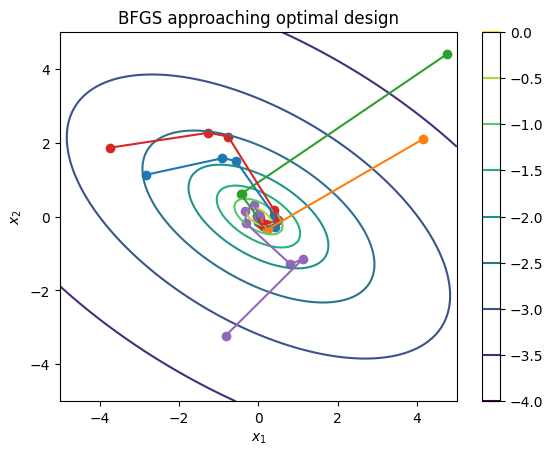
\includegraphics[width=0.8\textwidth]{week2/BFGS.png}
  \caption{BFGS algorithm optimizing for the most mutual information. The contours represent the mutual information.}
  \label{fig:BFGS}
\end{figure}
Running the BFGS algorithm 5 times with random start points over $I(\B{d})$ with $\Sigma_\theta=\begin{bmatrix}7.9 & 3 \\ 4 & 5\end{bmatrix}$ gives the plot seen in Figure \ref{fig:BFGS}. The algorithm usually converges after about 10 steps or so.
\subsection{Evaluation}
As it can be seen in Figure \ref{fig:BFGS}, the algorithm has no problem finding the optimal design for maximizing the mutual information between the prior and the posterior.
